\chapter{Implementation and Results}\label{ch:results}

\section{Implementation}

The system uses PyTorch, HuggingFace Transformers, \texttt{pytorch-crf}
and seqeval. \texttt{config.py} holds all settings,
\texttt{src/} holds the dataset and model code, and \texttt{train.py},
\texttt{evaluate.py} and \texttt{predict.py} handle training, testing and
inference. Two front ends are provided:
\begin{itemize}
  \item \textbf{Gradio web app} (\texttt{app.py}, Figure~\ref{fig:ui}):
  colour-coded entity highlighting, class filters, an entity table with
  confidence scores and Wikipedia/search links, distribution charts, and
  batch processing of text files with CSV export.
  \item \textbf{FastAPI service} (\texttt{server.py}): a \texttt{POST
  /predict} endpoint that returns entity spans and word-level tags as JSON.
\end{itemize}

\begin{figure}[H]
\centering
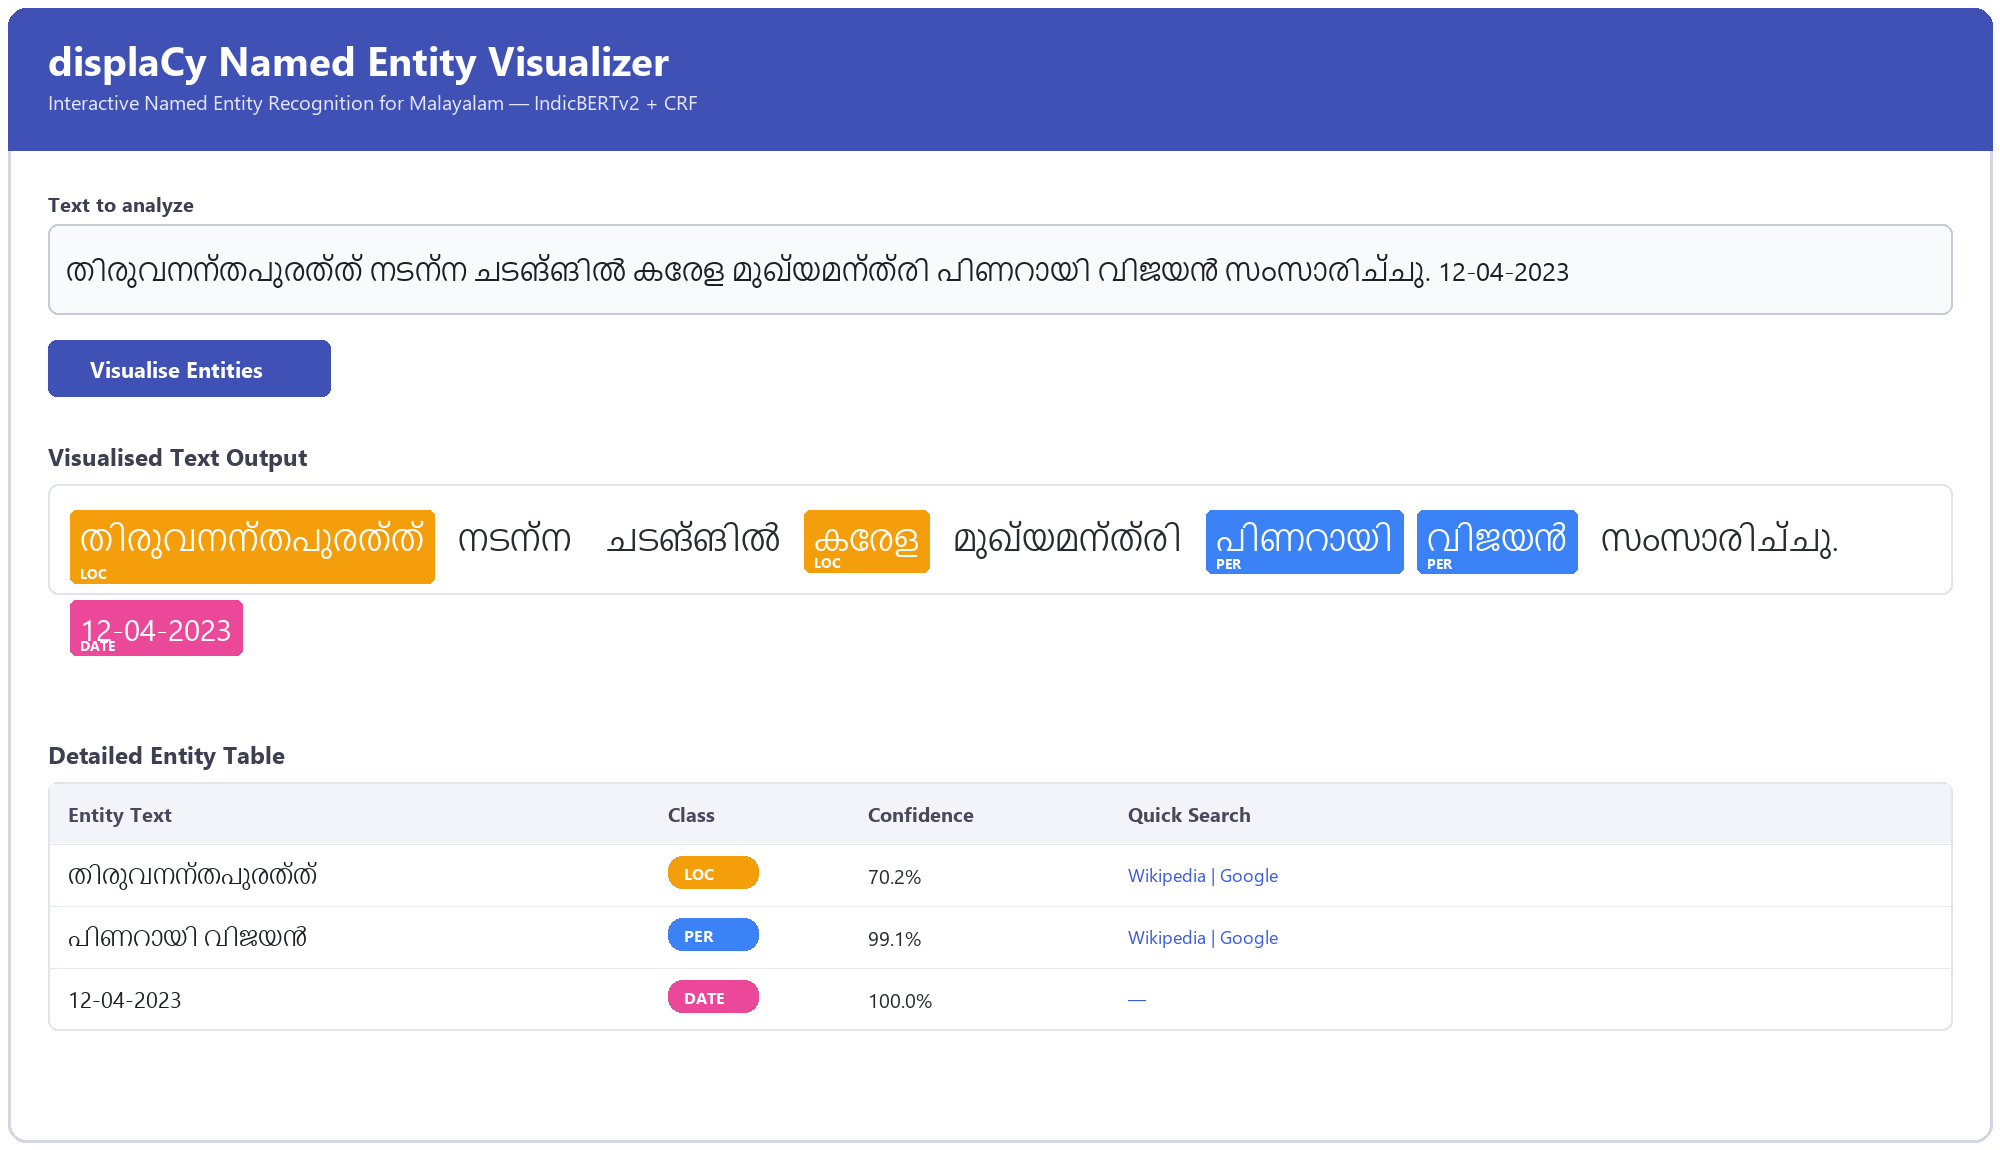
\includegraphics[width=0.9\textwidth]{demo_ui_mockup.png}
\caption{Web interface: \emph{Thiruvananthapuram} and \emph{Kerala} tagged as
LOC, \emph{Pinarayi Vijayan} as PER (99.1\%), and the date added by rules.}
\label{fig:ui}
\end{figure}

\section{Evaluation Metrics}

We report \textbf{strict entity-level} precision, recall and F1 with
seqeval. A predicted entity counts as correct only if its boundaries and
type both match the gold entity exactly:
\begin{equation}
P = \frac{TP}{TP+FP}, \qquad R = \frac{TP}{TP+FN}, \qquad F_1 = \frac{2PR}{P+R}.
\end{equation}
We also report token accuracy. All results are on the Naamapadam Malayalam
test set (965 sentences, 8{,}532 words, 1{,}505 entities).

\section{Softmax vs.\ CRF}

\begin{table}[H]
\centering
\caption{Strict entity-level results on the test set.}
\label{tab:entity}
\begin{tabular}{lccccccc}
\toprule
& & \multicolumn{3}{c}{Softmax (baseline)} & \multicolumn{3}{c}{CRF (proposed)} \\
\cmidrule(lr){3-5}\cmidrule(lr){6-8}
Entity & Support & P & R & F1 & P & R & F1 \\
\midrule
PER & 714 & 78.99 & 91.60 & 84.82 & 88.72 & 92.58 & \textbf{90.61} \\
LOC & 482 & 68.52 & 79.46 & 73.58 & 86.60 & 84.44 & \textbf{85.50} \\
ORG & 309 & 37.63 & 59.55 & 46.12 & 69.61 & 63.75 & \textbf{66.55} \\
\midrule
Micro avg & 1505 & 65.09 & 81.13 & 72.23 & 84.45 & 84.05 & \textbf{84.25} \\
Macro avg & 1505 & 61.71 & 76.87 & 68.17 & 81.64 & 80.26 & \textbf{80.89} \\
\midrule
Token accuracy & & \multicolumn{3}{c}{88.69} & \multicolumn{3}{c}{\textbf{94.08}} \\
Invalid IOB2 transitions & & \multicolumn{3}{c}{98} & \multicolumn{3}{c}{\textbf{20}} \\
\bottomrule
\end{tabular}
\end{table}

\begin{figure}[H]
\centering
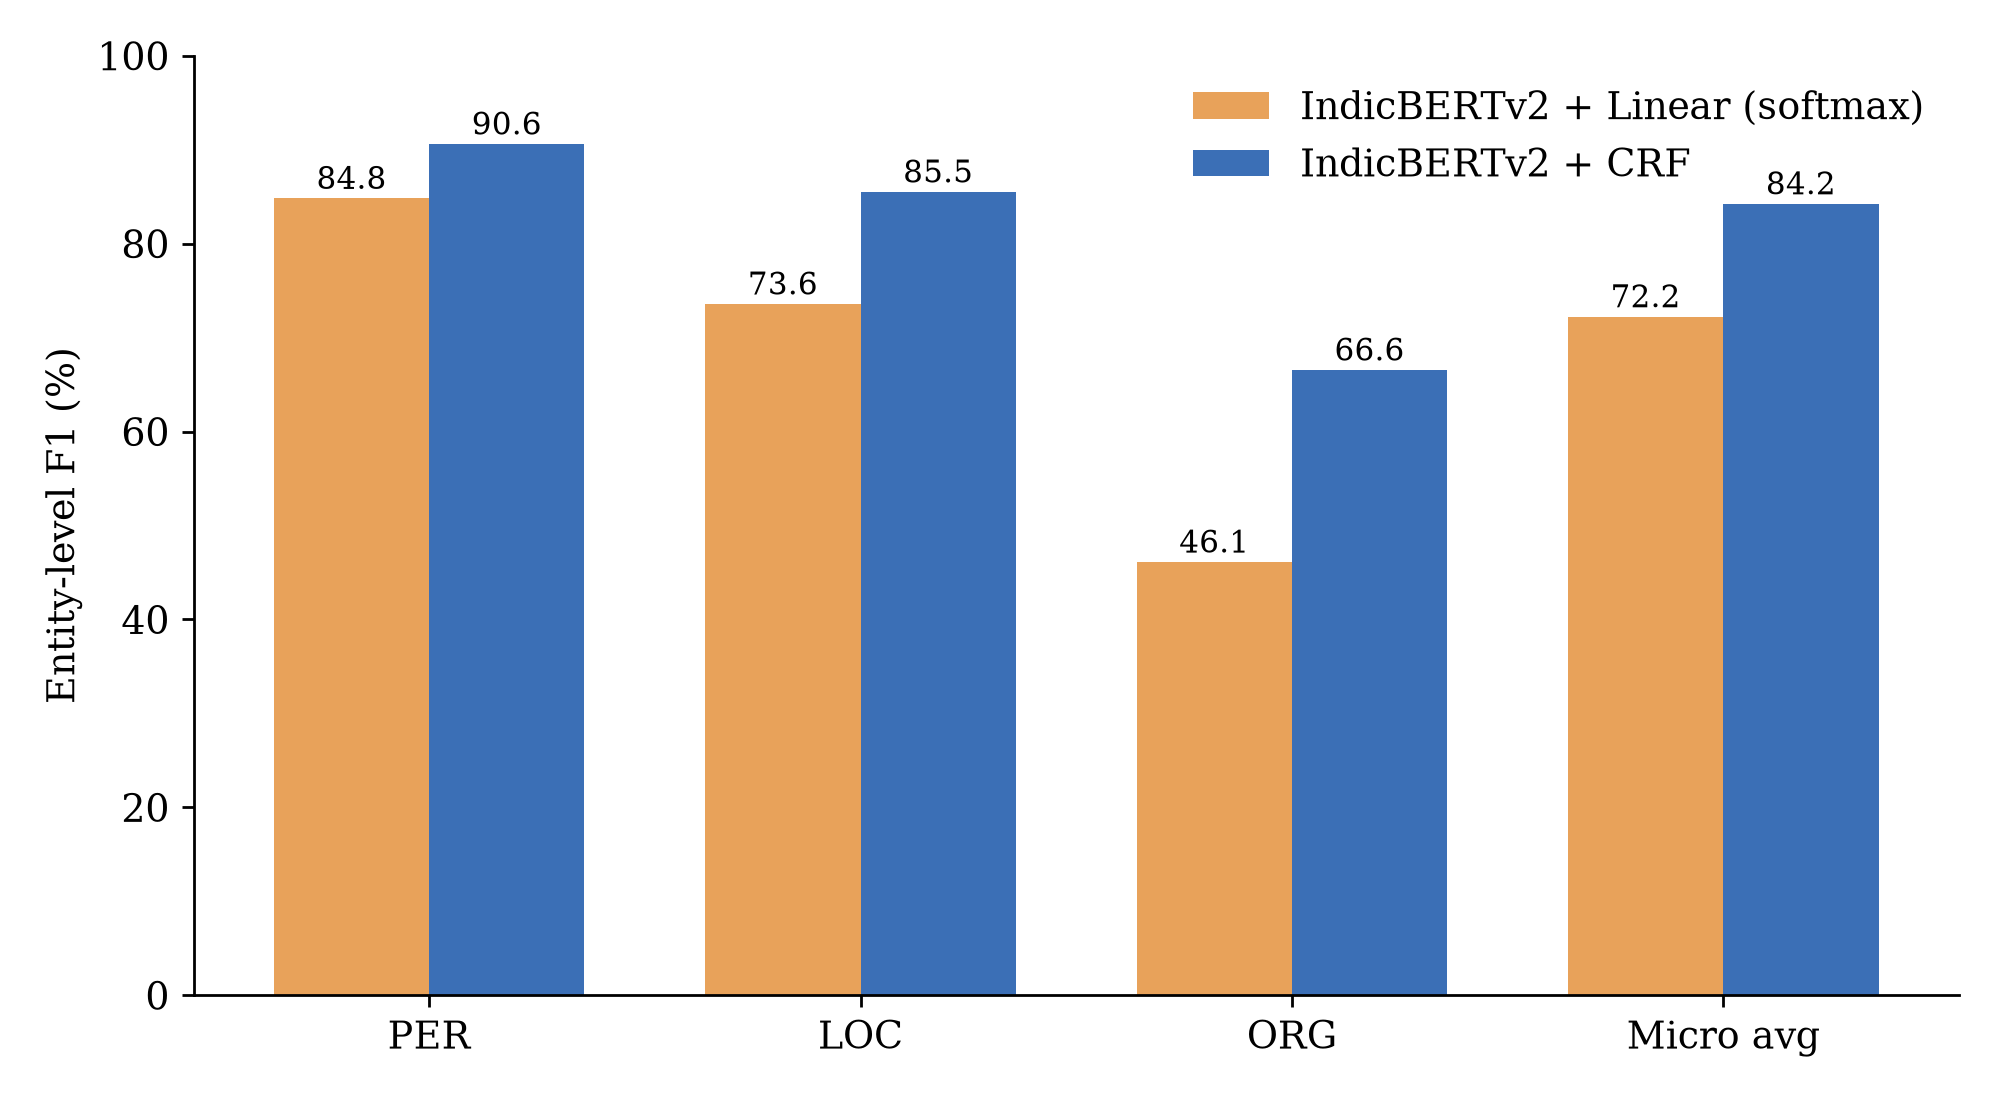
\includegraphics[width=0.75\textwidth]{f1_comparison.png}
\caption{Entity-level F1 per class.}
\label{fig:f1cmp}
\end{figure}

The CRF model is better on every class (Table~\ref{tab:entity},
Figure~\ref{fig:f1cmp}). Micro F1 rises by \textbf{12.0 points}, and the
largest gain is on ORG (+20.4), the class with the longest spans. The
softmax model has high recall but low precision. The class weights push it
to over-predict rare tags: 800 of the 6{,}051 \texttt{O} words are labelled
as entities, mostly \texttt{I-ORG} and \texttt{I-LOC}. The CRF is balanced
(P 84.5, R 84.1), and it reduces invalid transitions by 80\% at a cost of
about 20\% more inference time (8.3\,s vs.\ 6.9\,s for the test set on GPU).
Because the two models differ in both decoder and loss weighting, the gain
reflects both changes together.

\section{Error Analysis}

\begin{figure}[H]
\centering
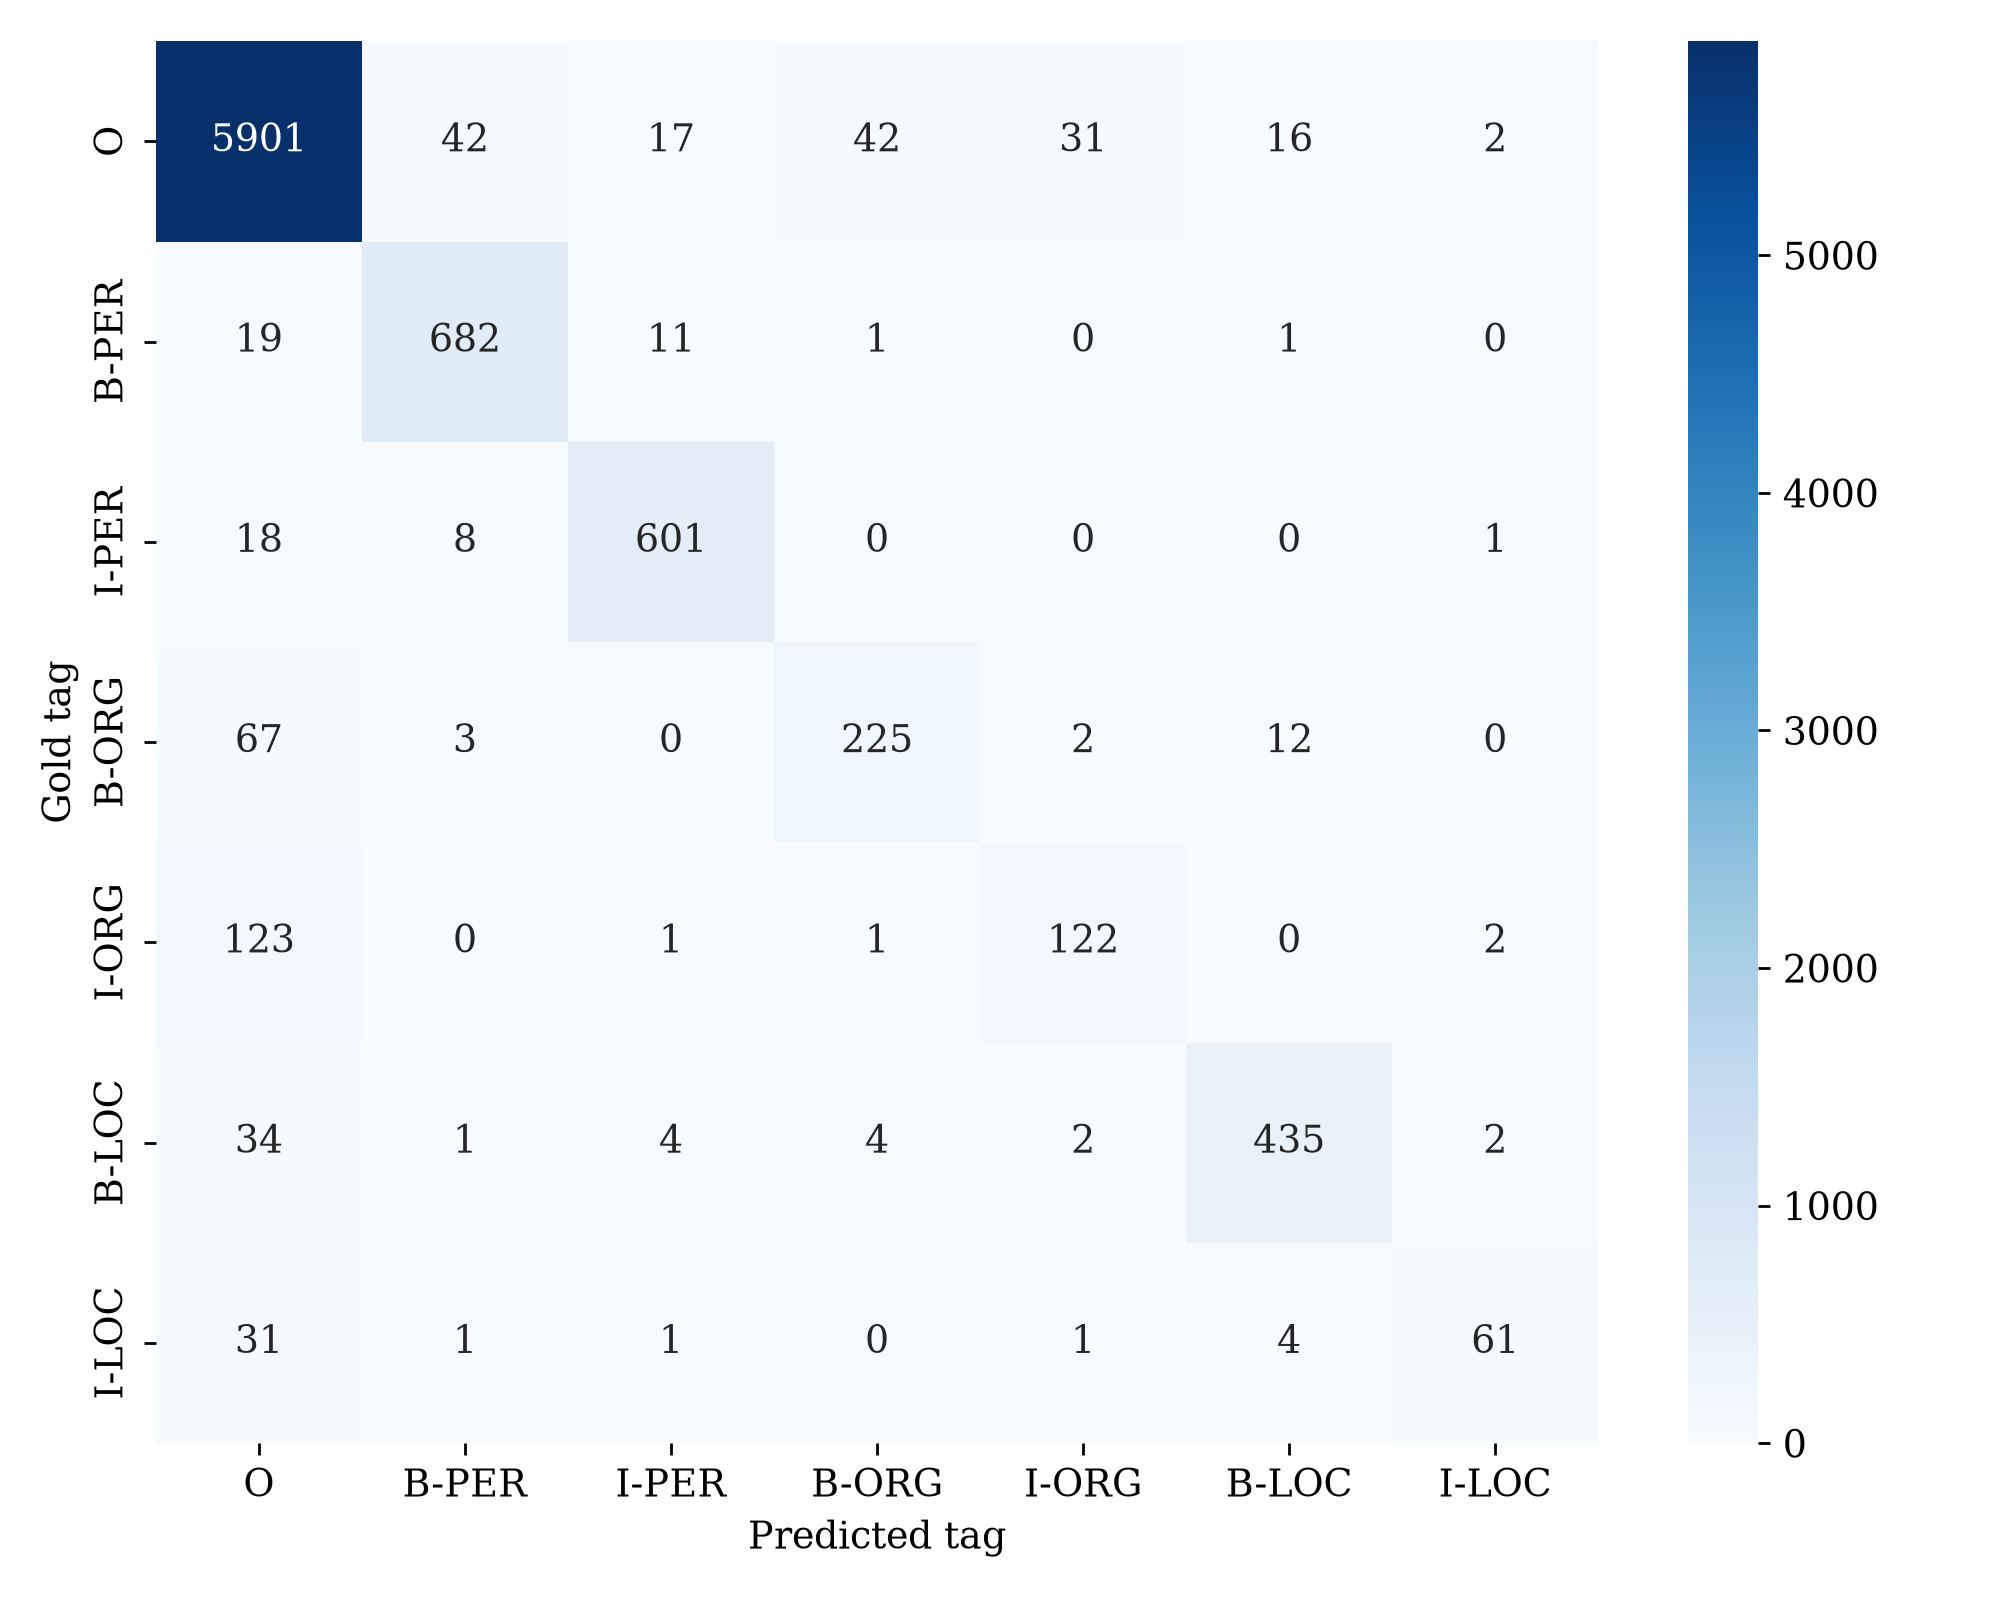
\includegraphics[width=0.62\textwidth]{cm_crf.png}
\caption{Token-level confusion matrix of the CRF model.}
\label{fig:cmcrf}
\end{figure}

Figure~\ref{fig:cmcrf} shows four main patterns:
\begin{itemize}
  \item \textbf{Detection, not typing, is the problem.} 292 entity words are
  predicted as \texttt{O}, but only 35 are confused with a different entity
  type.
  \item \textbf{ORG spans are truncated.} 123 of 249 \texttt{I-ORG} words
  are missed, so long organization names are often cut short. Under strict
  matching a truncated span counts as both an FP and an FN, which is why
  ORG entity F1 (66.6) is well below its \texttt{B-ORG} token F1 (77.3).
  \item \textbf{ORG/LOC ambiguity.} 12 \texttt{B-ORG} words are tagged
  \texttt{B-LOC}, since many organization names start with a place name.
  \item \textbf{Rare multi-word locations.} 31 of 99 \texttt{I-LOC} words
  are missed.
\end{itemize}

\section{Comparison with Published Work}

\begin{table}[H]
\centering
\caption{Comparison with published Malayalam NER results.}
\label{tab:lit}
\small
\begin{tabular}{llccc}
\toprule
System & Dataset & P (\%) & R (\%) & F1 (\%) \\
\midrule
Fuzzy SVM~\cite{lakshmi2016fuzzy} & In-house (500 sent.) & -- & -- & 88.13 \\
IndicNER (cited in~\cite{mohan2023finetuned}) & Naamapadam & -- & -- & 81.67 \\
Fine-tuned mBERT, base paper~\cite{mohan2023finetuned} & WikiAnn & 82.10 & 82.10 & 82.20 \\
Fine-tuned m-BERT~\cite{gopalakrishnan2025efficient} & Unreleased & 95.37 & 96.55 & 96.45 \\
\midrule
Ours: IndicBERTv2 + Softmax & Naamapadam & 65.09 & 81.13 & 72.23 \\
Ours: IndicBERTv2 + CRF & Naamapadam & 84.45 & 84.05 & \textbf{84.25} \\
\bottomrule
\end{tabular}
\end{table}

The datasets and protocols differ, so Table~\ref{tab:lit} is indicative
only. Our CRF model exceeds the base paper's Malayalam F1 (82.2) and the
IndicNER figure on the same benchmark (81.67), using 7\% of the training data
and strict span-level scoring. It shows the same class ranking as the base
paper (PER $>$ LOC $>$ ORG), which confirms that ORG is the hardest type.
The higher scores in~\cite{lakshmi2016fuzzy, gopalakrishnan2025efficient}
come from small or unreleased test sets and cannot be compared directly.
